\documentclass[border=12pt]{standalone}
\usepackage[utf8]{inputenc}
\usepackage[T1]{fontenc}
\usepackage{lmodern}
\usepackage{tikz}
\usetikzlibrary{positioning,fit,backgrounds,arrows.meta,shapes.multipart}

\definecolor{cCatBg}{HTML}{EEF7FC}
\definecolor{cCatBd}{HTML}{2A85BE}
\definecolor{cProBg}{HTML}{F0FAF4}
\definecolor{cProBd}{HTML}{206641}
\definecolor{cAteBg}{HTML}{FFF8EC}
\definecolor{cAteBd}{HTML}{B45309}
\definecolor{cHead}{HTML}{12405E}

\tikzset{
  tbl/.style={
    rectangle split, rectangle split parts=2,
    rectangle split part fill={#1, white},
    draw=#1, thick, rounded corners=2pt,
    align=left, font=\scriptsize\sffamily,
    inner sep=4pt, minimum width=3.75cm
  },
  zone/.style={
    rectangle, draw=#1, dashed, thick, rounded corners=6pt, inner sep=14pt
  },
  rel/.style={-{Stealth[length=2.2mm]}, thick, color=cHead},
  reld/.style={-{Stealth[length=2.2mm]}, thick, dashed, color=black!65},
  lbl/.style={font=\tiny\sffamily\bfseries, fill=white, inner sep=1.5pt}
}

\begin{document}
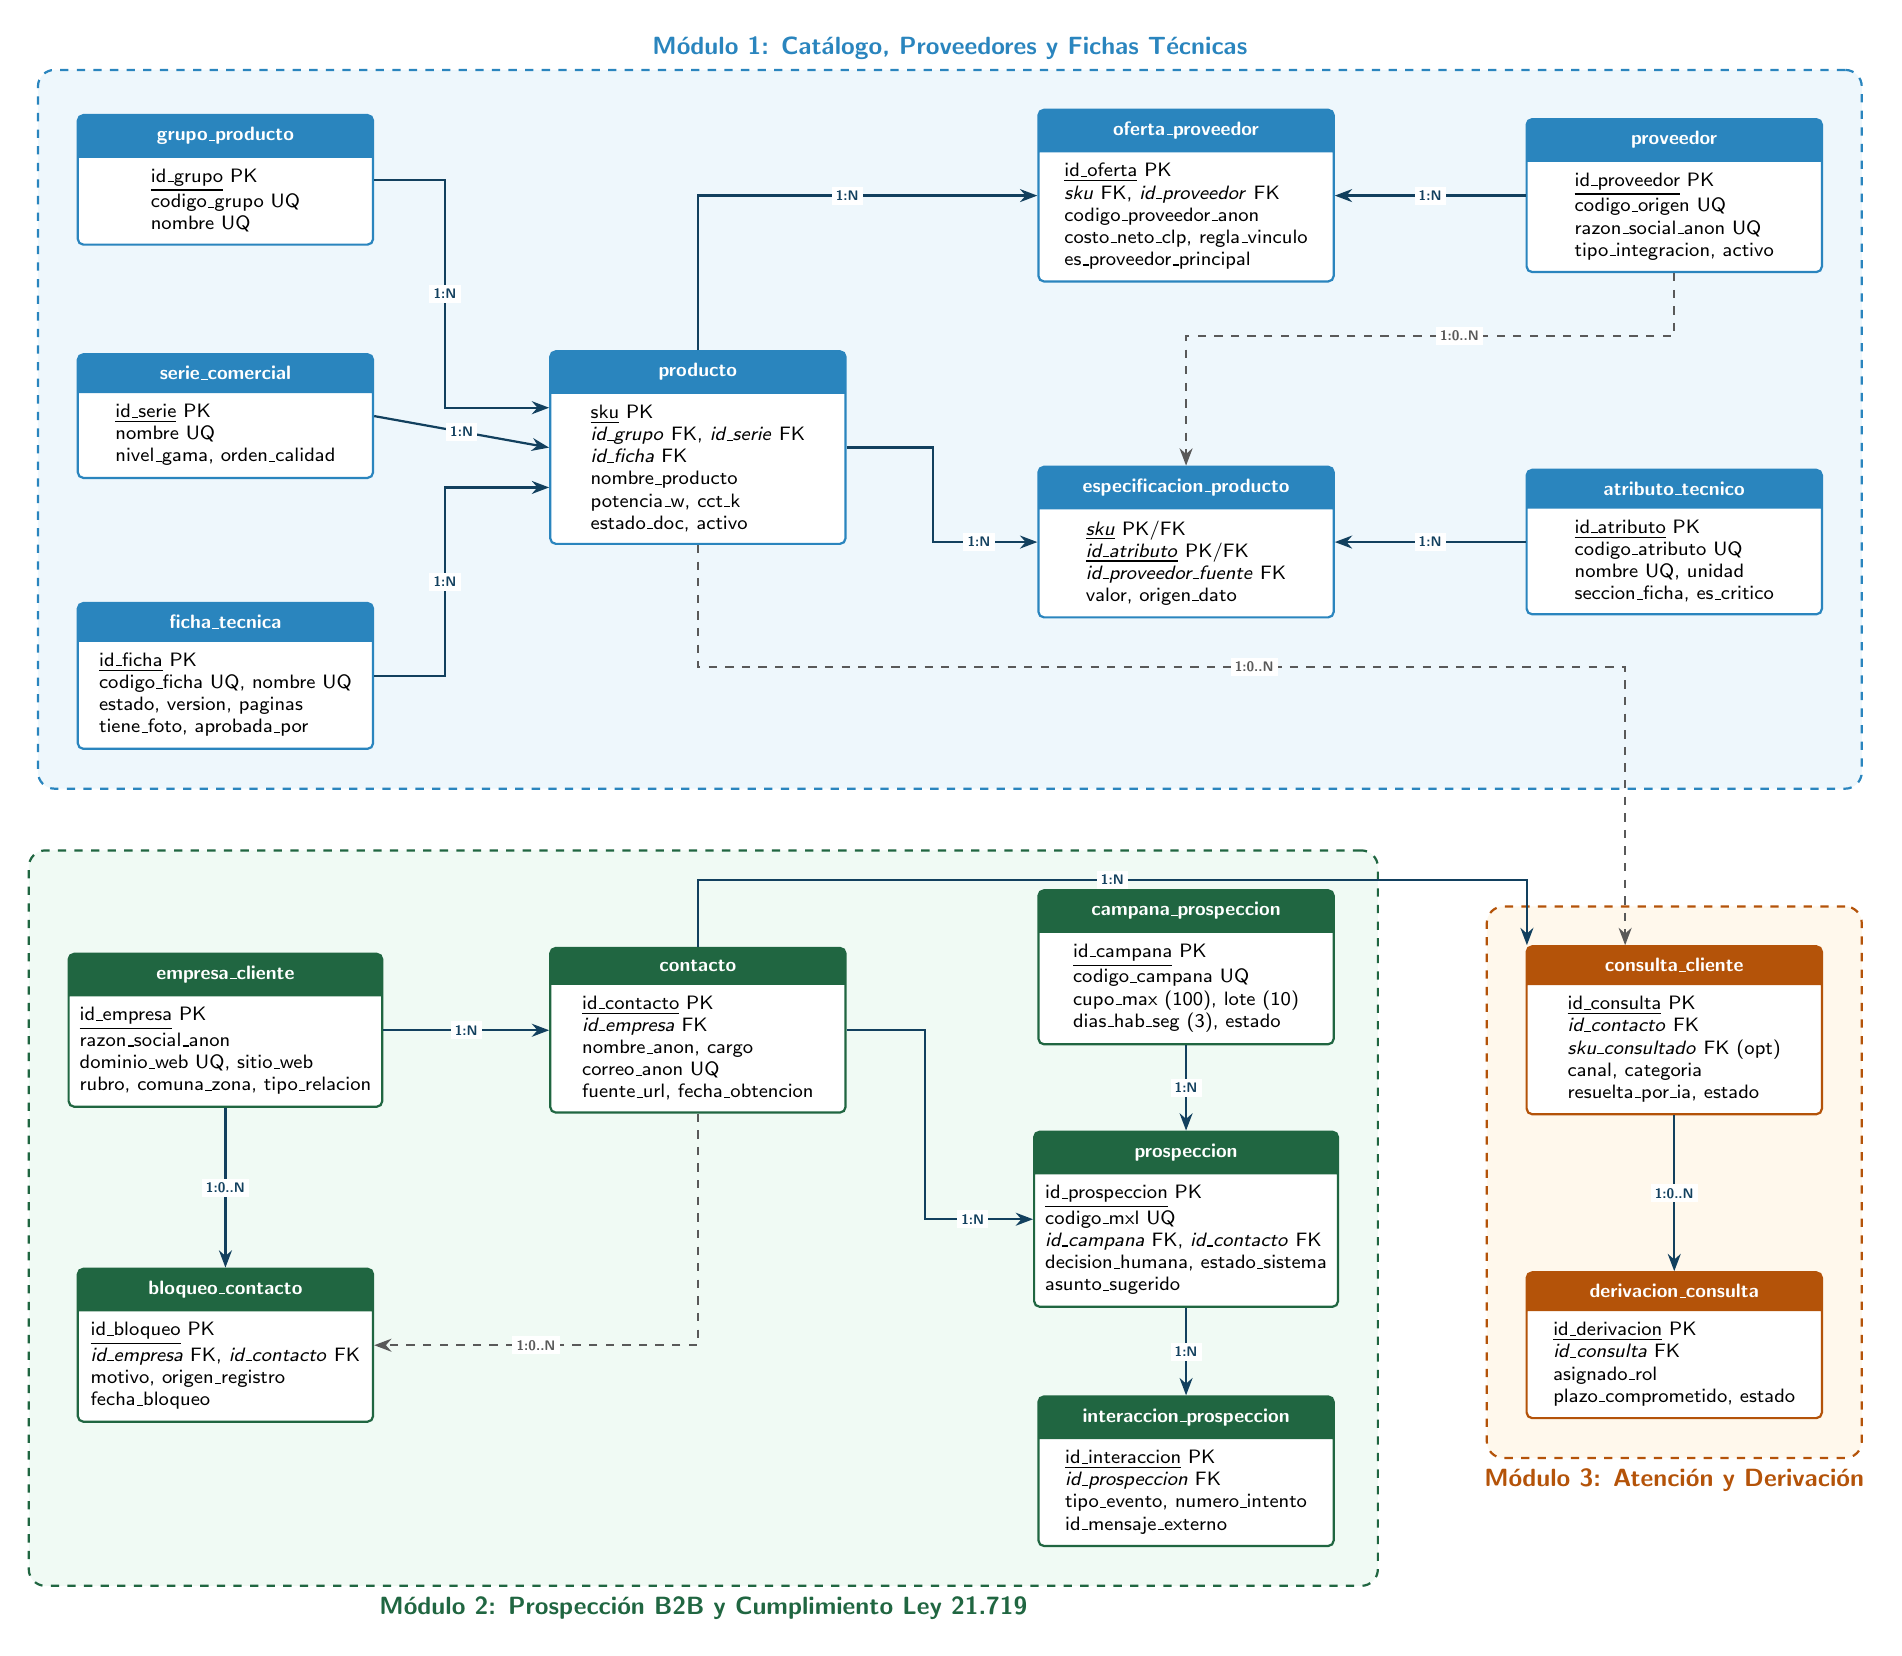
\begin{tikzpicture}

% --- MODULO 1: CATALOGO Y FICHAS (Y = 8.5 .. 15.5) ---
\node[tbl=cCatBd] (grupo) at (0, 15.2) {\textcolor{white}{\textbf{grupo\_producto}}\nodepart{two}\underline{id\_grupo} PK\\ codigo\_grupo UQ\\ nombre UQ};
\node[tbl=cCatBd] (serie) at (0, 12.2) {\textcolor{white}{\textbf{serie\_comercial}}\nodepart{two}\underline{id\_serie} PK\\ nombre UQ\\ nivel\_gama, orden\_calidad};
\node[tbl=cCatBd] (ficha) at (0, 8.9) {\textcolor{white}{\textbf{ficha\_tecnica}}\nodepart{two}\underline{id\_ficha} PK\\ codigo\_ficha UQ, nombre UQ\\ estado, version, paginas\\ tiene\_foto, aprobada\_por};

\node[tbl=cCatBd] (producto) at (6.0, 11.8) {\textcolor{white}{\textbf{producto}}\nodepart{two}\underline{sku} PK\\ \textit{id\_grupo} FK, \textit{id\_serie} FK\\ \textit{id\_ficha} FK\\ nombre\_producto\\ potencia\_w, cct\_k\\ estado\_doc, activo};

\node[tbl=cCatBd] (oferta) at (12.2, 15.0) {\textcolor{white}{\textbf{oferta\_proveedor}}\nodepart{two}\underline{id\_oferta} PK\\ \textit{sku} FK, \textit{id\_proveedor} FK\\ codigo\_proveedor\_anon\\ costo\_neto\_clp, regla\_vinculo\\ es\_proveedor\_principal};

\node[tbl=cCatBd] (prov) at (18.4, 15.0) {\textcolor{white}{\textbf{proveedor}}\nodepart{two}\underline{id\_proveedor} PK\\ codigo\_origen UQ\\ razon\_social\_anon UQ\\ tipo\_integracion, activo};

\node[tbl=cCatBd] (espec) at (12.2, 10.6) {\textcolor{white}{\textbf{especificacion\_producto}}\nodepart{two}\underline{\textit{sku}} PK/FK\\ \underline{\textit{id\_atributo}} PK/FK\\ \textit{id\_proveedor\_fuente} FK\\ valor, origen\_dato};

\node[tbl=cCatBd] (atrib) at (18.4, 10.6) {\textcolor{white}{\textbf{atributo\_tecnico}}\nodepart{two}\underline{id\_atributo} PK\\ codigo\_atributo UQ\\ nombre UQ, unidad\\ seccion\_ficha, es\_critico};

% --- MODULO 2: PROSPECCION B2B Y LEY 21.719 (Y = 0 .. 5.5) ---
\node[tbl=cProBd] (empresa) at (0, 4.4) {\textcolor{white}{\textbf{empresa\_cliente}}\nodepart{two}\underline{id\_empresa} PK\\ razon\_social\_anon\\ dominio\_web UQ, sitio\_web\\ rubro, comuna\_zona, tipo\_relacion};

\node[tbl=cProBd] (bloqueo) at (0, 0.4) {\textcolor{white}{\textbf{bloqueo\_contacto}}\nodepart{two}\underline{id\_bloqueo} PK\\ \textit{id\_empresa} FK, \textit{id\_contacto} FK\\ motivo, origen\_registro\\ fecha\_bloqueo};

\node[tbl=cProBd] (contacto) at (6.0, 4.4) {\textcolor{white}{\textbf{contacto}}\nodepart{two}\underline{id\_contacto} PK\\ \textit{id\_empresa} FK\\ nombre\_anon, cargo\\ correo\_anon UQ\\ fuente\_url, fecha\_obtencion};

\node[tbl=cProBd] (campana) at (12.2, 5.2) {\textcolor{white}{\textbf{campana\_prospeccion}}\nodepart{two}\underline{id\_campana} PK\\ codigo\_campana UQ\\ cupo\_max (100), lote (10)\\ dias\_hab\_seg (3), estado};

\node[tbl=cProBd] (prosp) at (12.2, 2.0) {\textcolor{white}{\textbf{prospeccion}}\nodepart{two}\underline{id\_prospeccion} PK\\ codigo\_mxl UQ\\ \textit{id\_campana} FK, \textit{id\_contacto} FK\\ decision\_humana, estado\_sistema\\ asunto\_sugerido};

\node[tbl=cProBd] (inter) at (12.2, -1.2) {\textcolor{white}{\textbf{interaccion\_prospeccion}}\nodepart{two}\underline{id\_interaccion} PK\\ \textit{id\_prospeccion} FK\\ tipo\_evento, numero\_intento\\ id\_mensaje\_externo};

% --- MODULO 3: ATENCION Y DERIVACIONES (DERECHA, Y = 0 .. 5.5) ---
\node[tbl=cAteBd] (consulta) at (18.4, 4.4) {\textcolor{white}{\textbf{consulta\_cliente}}\nodepart{two}\underline{id\_consulta} PK\\ \textit{id\_contacto} FK\\ \textit{sku\_consultado} FK (opt)\\ canal, categoria\\ resuelta\_por\_ia, estado};

\node[tbl=cAteBd] (deriv) at (18.4, 0.4) {\textcolor{white}{\textbf{derivacion\_consulta}}\nodepart{two}\underline{id\_derivacion} PK\\ \textit{id\_consulta} FK\\ asignado\_rol\\ plazo\_comprometido, estado};

% --- FONDOS DE MODULO ---
\begin{scope}[on background layer]
  \node[zone=cCatBd, fill=cCatBg, fit=(grupo)(serie)(ficha)(producto)(oferta)(prov)(espec)(atrib), label={[font=\small\bfseries\sffamily, text=cCatBd]above:Módulo 1: Catálogo, Proveedores y Fichas Técnicas}] (z1) {};
  \node[zone=cProBd, fill=cProBg, fit=(empresa)(contacto)(bloqueo)(prosp)(campana)(inter), label={[font=\small\bfseries\sffamily, text=cProBd]below:Módulo 2: Prospección B2B y Cumplimiento Ley 21.719}] (z2) {};
  \node[zone=cAteBd, fill=cAteBg, fit=(consulta)(deriv), label={[font=\small\bfseries\sffamily, text=cAteBd]below:Módulo 3: Atención y Derivación}] (z3) {};
\end{scope}

% --- RELACIONES MODULO 1 ---
\draw[rel] (grupo.east) -- ++(0.9,0) |- node[lbl, pos=0.25]{1:N} (producto.165);
\draw[rel] (serie.east) -- node[lbl, midway]{1:N} (producto.west);
\draw[rel] (ficha.east) -- ++(0.9,0) |- node[lbl, pos=0.25]{1:N} (producto.195);
\draw[rel] (producto.north) |- node[lbl, pos=0.72]{1:N} (oferta.west);
\draw[rel] (prov.west) -- node[lbl, midway]{1:N} (oferta.east);
\draw[rel] (producto.east) -- ++(1.1,0) |- node[lbl, pos=0.72]{1:N} (espec.west);
\draw[rel] (atrib.west) -- node[lbl, midway]{1:N} (espec.east);
\draw[reld] (prov.south) -- ++(0,-0.8) -| node[lbl, pos=0.22]{1:0..N} (espec.north);

% --- RELACIONES MODULO 2 ---
\draw[rel] (empresa.east) -- node[lbl, midway]{1:N} (contacto.west);
\draw[rel] (empresa.south) -- node[lbl, midway]{1:0..N} (bloqueo.north);
\draw[reld] (contacto.south) |- node[lbl, pos=0.75]{1:0..N} (bloqueo.east);
\draw[rel] (contacto.east) -- ++(1.0,0) |- node[lbl, pos=0.72]{1:N} (prosp.west);
\draw[rel] (campana.south) -- node[lbl, midway]{1:N} (prosp.north);
\draw[rel] (prosp.south) -- node[lbl, midway]{1:N} (inter.north);

% --- RELACIONES MODULO 3 ---
\draw[rel] (contacto.north) -- ++(0,0.85) -| node[lbl, pos=0.25]{1:N} (consulta.150);
\draw[reld] (producto.south) -- ++(0,-1.55) -| node[lbl, pos=0.3]{1:0..N} (consulta.120);
\draw[rel] (consulta.south) -- node[lbl, midway]{1:0..N} (deriv.north);

\end{tikzpicture}
\end{document}
